\documentclass[a4paper,12pt]{article}
\usepackage[margin=2cm]{geometry}

%\usepackage[T1]{fontenc}
%\usepackage [isolatin]{inputenc}
\usepackage{graphicx}
\usepackage{listings}

\begin{document}

\title{\textbf{Cats short notice}}
\author{Pierre Morfouace\\
        \texttt{morfouac@ipno.in2p3.fr}\\
        version 1.0
}
\maketitle 

\tableofcontents
\pagebreak


\section{Brief description of Cats detector}
~\\
\indent Beams produced by fragmentation have a large emittance. In order to know the position of interaction on the target and the beam angle event by event with a precision good enough we have used two beam tracking detectors. In addition, these detectors are also used to count the incident beam and provide us a good time information.\\
In the experiment, we have used two CATS\footnote{Chambre \`A Trajectoire de Saclay} detectors \cite{Ott}. This detector is a low pressure multi-wire proportional chamber (figure \ref{fig:CATS}) used with an isobutane gas ($C_4H_{10}$). The gas pressure depends on the ion beam and the pressure used in our experiment was 10 mbar. The active area of this detector is $70 \times 70$ mm$^2$. There are two Mylar foils 1.5 $\mu$m thick that contain the gas inside. Each detector is made of an anode that is a plane of 71 anode wires in tungsten which have a diameter of 10 $\mu$m and there is 1 mm between each wire. In this anode plane we put a high voltage between 600 and 800 V. Either side of the anode there are two cathode planes at a distance of 3.2 mm which are perpendicular between them. The fact that the cathode is segmented provides us with the position information. Each cathode contains 28 gold strips spaced by 0.2 mm and 2.34 mm thick. Then we are able to reconstruct the beam position on the target event by event with a precision less than 1 mm.\\
The maximum count rate for this detector is about $10^5$ particles per second if the beam is not too focused on one part of the detector.
\begin{figure}[h!]
\begin{center}
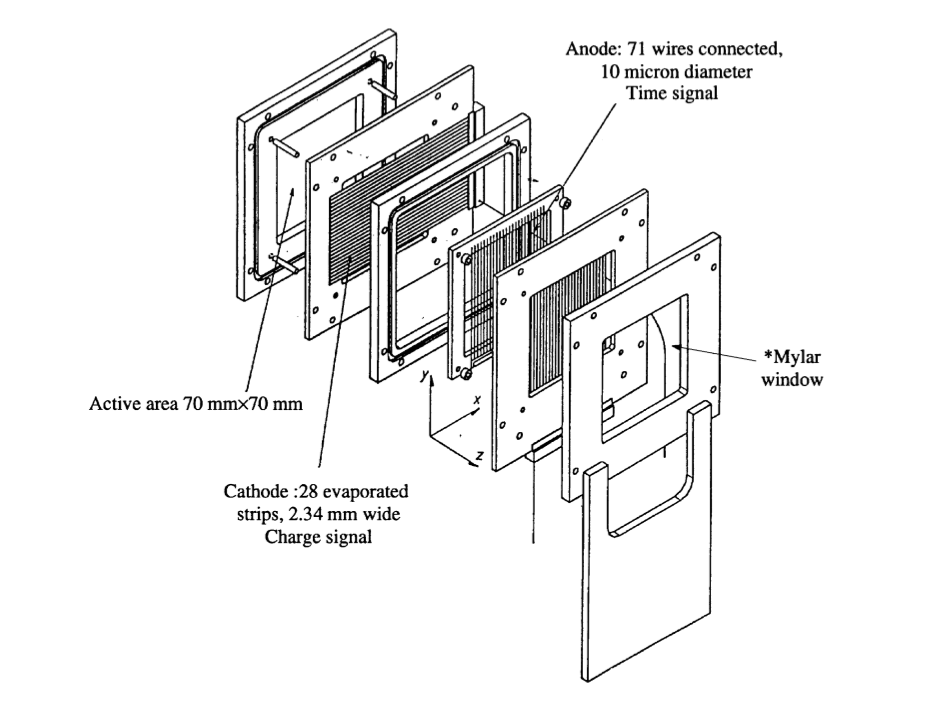
\includegraphics[scale=0.35]{CATS_det.png}
\caption{\textit{Characteristics of a CATS detector}}
\label{fig:CATS}
\end{center}
\end{figure}

\section{Description of geometry file}
Including a CATS detector in NPTool is as easy as including the following
lines in your *.detector file:
\begin{verbatim}
CATSArray
CATSDetector
   X1_Y1=          -34.36  -34.96  -1193
   X28_Y1=         36.76   -34.96  -1193
   X1_Y28=         -34.36  36.16   -1193
   X28_Y28=        36.76   36.16   -1193
\end{verbatim}
This geometry file corresponds to the coordinate $(X,Y,Z)$ in that order for the fours corners of the CATS detector.

\section{Description of configuration options}
The config file is located in ./configs/ConfigCATS.dat and its typical structure is as following:
\begin{verbatim}
configCATS
% DISABLE CHANNEL (if needed)
	DISABLE_CHANNEL CATS1STRX1
	DISABLE_CHANNEL CATS2STRY28

% INVERSION CHANNEL
	INVERSION CATS1 STRY14 STRY6
	INVERSION CATS2 STRX15 STRX16
	
% RECONSTUCTION_METHOD: 4 reconstruction are available
% FSECH: for fitted hyperbolic secante method 
% ASECH: for analytic hyperbolic secante method
% AGAUSS: for analytic Gaussian method
% CENTROIDE: for a simple centroid method
RECONSTUCTION_METHOD CATS1X FSECH
RECONSTUCTION_METHOD CATS1Y FSECH
RECONSTUCTION_METHOD CATS2X FSECH
RECONSTUCTION_METHOD CATS2Y FSECH
\end{verbatim}
When the line begins with \%, it means that it is a comment. Here is listed the different token.
\begin{itemize}
   \item DISABLE\_CHANNEL: some strip can be missing or can burn during the experiment and then it is needed to remove it for the analysis. This is done with this token by specifying the detector number and the strip.
   \item INVERSION / STRX / STRY: it is also possible that electronically two strips are switched. In order to deal with this problem we use the INVERSION token by specifying first the detector we are talking about and then the two strips we need to invert.
   \item RECONSTRUCTION\_METHOD: different method are possible to use to reconstruct the position of the beam on CATS detector. The main one is the secant hyperbolic that we can use by fitting the charge distribution or we can also use the analytic method that take the three highest charge. The analytical Gaussian method is also available and is very similar to the analytical secant method. Finally we can also chose the barycentric method by choosing the centroids method that correspond to the barycenter of the charge distribution.
\end{itemize}

\section{Physical treatment of Cats detector}
Each event are treated in the function BuildPhysicalEvent of TCATSPhysics.cxx. For each event, we determine the detecter number, the strips number and for each strip the associated charge. We reconstruct the position of the beam with the method chosen in the RECONSTRUCTION\_METHOD.\\
We usually have two detectors in an experiment to reconstruct the position of the beam on the target. After knowing the position of the beam on both detectors we project it on the target to have event by event the position of interaction. To do so, we need the distance between the two CATS and between the CATS and the target. This information is know from the geometry file, since the $Z$ position corresponds to the distance in mm between the target and the detector. Then event by event we have the position on the target and the beam direction.

\section{Example of simple analysis}
\subsection{Running the analysis}
The following command line should be executed:

\begin{verbatim}
   ./Analysis -D yyy.detector -R RunToTreat.txt -C calibration.txt
\end{verbatim}

where yyy.detector is the input file describing the detector geometry used in NPSimulation. All these input files are based on keywords and can be found  in the \$NPTool/Inputs subdirectories. The RunToTreat.txt file contains the name of the files (either from NPSimulation or from real experiment) which should be analysed. The name of the tree should also be specified. An example of such a file is given here:

\begin{verbatim}
   TTreeName
           AutoTree
   RootFileName
	../../NPData/cats_mask_e644.root
\end{verbatim}


\subsection{Results of the analysis}
The results of the anaysis are stored in a ROOT file in the \$NPTool/Output/Analysis
directory. 

The results you should obtain are displayed in the following Figures. Run the 
ShowResult.C macro in order to get them.

\begin{thebibliography}{99}
\bibitem{Ott} S. Ottini {\it et al.} {\it Nucl. Instr. and Meth. in Phys. Res.} A {\bf 431} 476 (1999).
\end{thebibliography}

\end{document}

